\section{Scope Inference}
\label{sec:inference}

The broker infers $S(t)$ from the task text before the agent starts (Algorithm~\ref{alg:infer}). It combines a
language-model proposal with deterministic steps whose behaviour can be tested and audited.

\textbf{Semantic layer.} For each database the broker builds a semantic layer automatically from the catalog
(tables, columns, types, declared keys, row counts) and from dataset-provided metadata: BIRD column
descriptions and foreign keys from the official PostgreSQL schema file, and Spider natural-language column
names and keys from \texttt{tables.json}. Example values that appear in those files are discarded, so no data
value reaches any prompt. Nothing is written by hand for an individual database.

\textbf{LLM proposal.} An inference model receives the rendered schema and the task and returns, under a JSON
schema constraint, the tables the query must read (including bridge tables), the needed columns, and row
filters stated in the task with a literal value. The inference model runs on the broker side; it is a small
open-weight model in our evaluation (Section~\ref{sec:setup}).

\textbf{Schema linking.} A deterministic lexical linker adds tables whose name tokens all occur in the task, and
columns of included tables whose name tokens occur in the task (strict) or whose name or description tokens
overlap sufficiently (lenient).

\textbf{Grounding of row filters.} A proposed filter is kept only if every literal value occurs verbatim
(case-insensitive) in the task text, so the inference model cannot invent row restrictions the task does not
state. Text equality is compiled case-insensitively.

\textbf{Conservativeness $k$.} $k$ trades exposure for robustness and is monotone ($S_0\sqsubseteq S_1\sqsubseteq S_2$):
$k{=}0$ keeps the proposal, strict links and all grounded filters; $k{=}1$ adds lenient links and every key
column of every included table, and keeps only equality and \texttt{IN} filters (range filters are dropped,
but their columns remain); $k{=}2$ keeps every column of every included table and no task filter.

\textbf{FK closure.} Tables are connected through shortest foreign-key paths (a greedy Steiner approximation);
intermediate tables and the join columns of every hop are added.

\textbf{Intersection with $E(u)$.} Columns outside the entitlement are removed, as are task predicates that
mention them. Row entitlement is not re-implemented by the broker: it is enforced by the database through view
ownership (Section~\ref{sec:enforcement}).

\begin{algorithm}[t]
\caption{Task-scope inference (broker side)}
\label{alg:infer}
\begin{algorithmic}[1]
\REQUIRE task text $x$, semantic layer $L$, entitlement $E$, conservativeness $k$
\STATE $P \leftarrow \textsc{LLMPropose}(L.\textsc{render}(), x)$ \COMMENT{tables, columns, filters}
\STATE $T \leftarrow P.\mathit{tables}\cup \mathrm{tables}(P.\mathit{cols}) \cup \textsc{LinkTables}(x,L)$
\STATE $C \leftarrow P.\mathit{cols}\cup\textsc{LinkCols}(x,L,T,\mathit{lenient}{=}(k\ge1))$
\IF{$k\ge1$} \STATE $C\leftarrow C\cup\{\text{key columns of } T\}$ \ENDIF
\IF{$k=2$} \STATE $C\leftarrow C\cup\{\text{all columns of } T\}$ \ENDIF
\STATE $\Phi\leftarrow\emptyset$
\FORALL{$f\in P.\mathit{filters}$ with $\textsc{Grounded}(f.\mathit{value},x)$}
  \STATE $C\leftarrow C\cup\{f.\mathit{column}\}$
  \IF{$k=0$ \OR ($k=1$ \AND $f.\mathit{op}\in\{=,\textsc{in}\}$)} \STATE $\Phi\leftarrow\Phi\cup\{f\}$ \ENDIF
\ENDFOR
\STATE $S\leftarrow \textsc{FKClosure}(\textsc{Scope}(C,\Phi),L)$
\RETURN $S\sqcap_{\mathrm{cols}} E$
\end{algorithmic}
\end{algorithm}

All deterministic steps (tokenization, linking, grounding, filter compilation, monotonicity in $k$, FK closure,
intersection) are covered by unit tests in the artifact. Their cost is linear in the schema size and negligible
next to the model call.

\section{Enforcement and Widening}
\label{sec:enforcement}

\begin{figure*}[t]
\centering
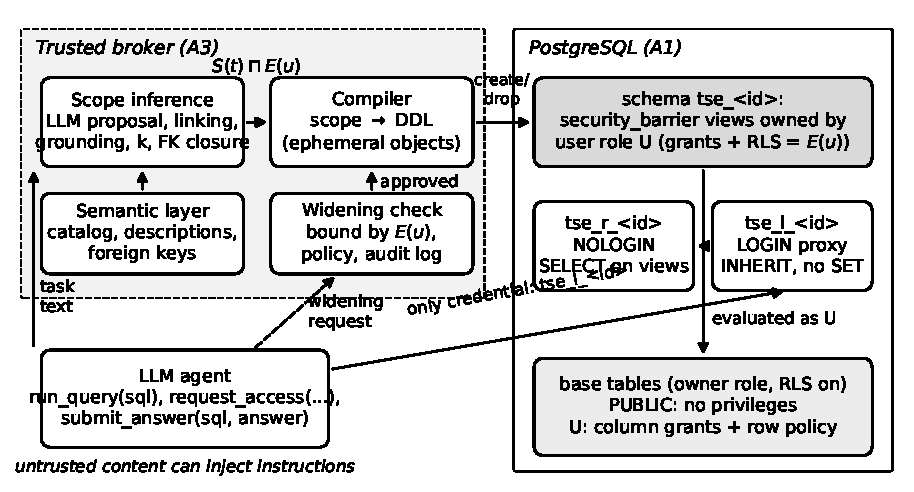
\includegraphics[width=0.85\textwidth]{figs/architecture.pdf}
\caption{TSE architecture. The trusted broker infers $S(t)$, compiles it into an ephemeral schema of
\texttt{security\_barrier} views owned by the user role $U$ and an ephemeral login, and tears everything
down at task end. The agent's only credential is the ephemeral login; widening requests go to the broker,
which bounds them by $E(u)$, applies the approval policy and logs them.}
\label{fig:arch}
\end{figure*}

\subsection{Compilation}
Fig.~\ref{fig:arch} shows the architecture. Base tables are owned by a dedicated owner role and have row-level
security enabled. Each user role $U$ holds column-level \texttt{SELECT} grants and one permissive \texttt{SELECT}
policy per table, which together implement $E(u)$. For each task the broker, a non-superuser role with
\texttt{CREATEROLE}, executes the DDL of Listing~\ref{lst:ddl} in one transaction:
\begin{enumerate}
\item create schema \texttt{tse\_<id>};
\item while acting as $U$ (the broker may \texttt{SET ROLE} to $U$ but does not inherit its privileges), create one
\texttt{security\_barrier} view per scoped table, selecting the scoped columns and applying the task predicate.
Because $U$ owns the views, PostgreSQL evaluates them with $U$'s column grants and $U$'s row policy;
\item create a \texttt{NOLOGIN} role \texttt{tse\_r\_<id>} with \texttt{USAGE} on the schema and \texttt{SELECT}
on its views, and a login proxy \texttt{tse\_l\_<id>} that is a member of it \texttt{WITH INHERIT TRUE, SET FALSE};
\item pin the login's \texttt{search\_path} to the task schema, make its transactions read-only and set a statement
timeout.
\end{enumerate}
\texttt{PUBLIC} holds no privileges on the database, on schema \texttt{public}, or on base tables, and
temporary-object creation is revoked. At task end the broker terminates the login's sessions and drops the schema
and both roles; a sweep removes leftovers idempotently. The agent sees the scoped schema, including the task row
filters (non-Truman transparency~\cite{rizvi2004extending}), so it knows which rows it can see and can request
more.

\begin{figure}[t]
\footnotesize
\begin{verbatim}
CREATE SCHEMA tse_9f2c;
GRANT USAGE, CREATE ON SCHEMA tse_9f2c TO u_role;
SET ROLE u_role;      -- views owned by the user role
CREATE VIEW tse_9f2c.singer
  WITH (security_barrier = true) AS
  SELECT "name","country","singer_id"
  FROM public.singer
  WHERE lower("country"::text) = lower('France');
RESET ROLE;
REVOKE CREATE ON SCHEMA tse_9f2c FROM u_role;
CREATE ROLE tse_r_9f2c NOLOGIN;
GRANT USAGE ON SCHEMA tse_9f2c TO tse_r_9f2c;
SET ROLE u_role;
GRANT SELECT ON ALL TABLES IN SCHEMA tse_9f2c
  TO tse_r_9f2c;
RESET ROLE;
CREATE ROLE tse_l_9f2c LOGIN PASSWORD '...';
GRANT tse_r_9f2c TO tse_l_9f2c
  WITH INHERIT TRUE, SET FALSE;
ALTER ROLE tse_l_9f2c IN DATABASE db
  SET search_path = tse_9f2c;
ALTER ROLE tse_l_9f2c IN DATABASE db
  SET default_transaction_read_only = on;
\end{verbatim}
\caption{Compiled DDL for a one-table scope (identifiers shortened).}
\label{lst:ddl}
\end{figure}

\subsection{Widening protocol}
\label{sec:widening}
When the scope is insufficient, the agent calls \texttt{request\_access} with specific \texttt{table.column}
names and/or tables whose task filter should be removed, plus a reason. The broker: (1)~\emph{bounds} the
request: items outside $E(u)$ are rejected and logged as exceeding the entitlement (they could not be granted
anyway, because the view owner lacks the privilege); (2)~\emph{decides} the in-bound part with an approval policy;
(3)~\emph{applies} approved items by replacing the affected views (columns are only appended; predicates only
relaxed); and (4)~\emph{audits} the request, the decision and the resulting scope. We evaluate three simulated
approval policies: \emph{auto} (approve in-bound items with a non-empty reason, at most three approved requests
per task), \emph{strict} (as auto, but deny columns tagged sensitive by a fixed lexical tagger, modeling a
cautious user), and \emph{deny} (no widening; ablation). Widening converts an inference error from a task failure
into a bounded, auditable request. It also opens a channel an attacker can try to use, which we measure in
Section~\ref{sec:res-security}.
